\documentclass[a4paper,12pt]{llncs}
\usepackage{fullpage}
\usepackage[british]{babel}
\usepackage[T1]{fontenc}
\usepackage{amsmath}
\usepackage{amssymb}
\usepackage[T1]{fontenc}
\usepackage[latin1]{inputenc} 
%\usepackage{amsthm} \newtheorem{theorem}{Theorem}
\usepackage{color}
\usepackage{float}


\usepackage{dot2texi}
\usepackage{tikz}

\usetikzlibrary{calc,trees,positioning,arrows,chains,shapes.geometric,%
    decorations.pathreplacing,decorations.pathmorphing,shapes,%
    matrix,shapes.symbols}


\tikzset{
>=stealth',
  punktchain/.style={
    rectangle, 
    rounded corners, 
    % fill=black!10,
    draw=black, very thick,
    text width=10em, 
    minimum height=3em, 
    text centered, 
    on chain},
  line/.style={draw, thick, <-},
  element/.style={
    tape,
    top color=white,
    bottom color=blue!50!black!60!,
    minimum width=8em,
    draw=blue!40!black!90, very thick,
    text width=10em, 
    minimum height=3.5em, 
    text centered, 
    on chain},
  every join/.style={->, thick,shorten >=1pt},
  decoration={brace},
  tuborg/.style={decorate},
  tubnode/.style={midway, right=2pt},
}

\usepackage{caption}
\DeclareCaptionFont{white}{\color{white}}
\DeclareCaptionFormat{listing}{\colorbox{gray}{\parbox{\textwidth}{#1#2#3}}}
\captionsetup[lstlisting]{format=listing,labelfont=white,textfont=white}


\usepackage{alltt}
\usepackage{listings}
 \usepackage{aeguill} 
\usepackage{dsfont}
%\usepackage{algorithm}
\usepackage[noend]{algorithm2e}
%\usepackage{algorithmicx}
\usepackage{subfig}
\lstset{% parameters for all code listings
	language=Python,
	frame=single,
	basicstyle=\small,  % nothing smaller than \footnotesize, please
	tabsize=2,
	numbers=left,
	framexleftmargin=2em,  % extend frame to include line numbers
	%xrightmargin=2em,  % extra space to fit 79 characters
	breaklines=true,
	breakatwhitespace=true,
	prebreak={/},
	captionpos=b,
	columns=fullflexible,
	escapeinside={\#*}{\^^M}
}


\usepackage{fancyvrb}
\DefineVerbatimEnvironment{code}{Verbatim}{fontsize=\small}
\DefineVerbatimEnvironment{example}{Verbatim}{fontsize=\small}

\usepackage{url}
\urldef{\mailsa}\path|sharyari@gmail.com |    
\newcommand{\keywords}[1]{\par\addvspace\baselineskip
\noindent\keywordname\enspace\ignorespaces#1}


\usepackage{tikz} \usetikzlibrary{trees}
\usepackage{hyperref}  % should always be the last package

% useful colours (use sparingly!):
\newcommand{\blue}[1]{{\color{blue}#1}}
\newcommand{\green}[1]{{\color{green}#1}}
\newcommand{\red}[1]{{\color{red}#1}}

% useful wrappers for algorithmic/Python notation:
\newcommand{\length}[1]{\text{len}(#1)}
\newcommand{\twodots}{\mathinner{\ldotp\ldotp}}  % taken from clrscode3e.sty
\newcommand{\Oh}[1]{\mathcal{O}\left(#1\right)}

% useful (wrappers for) math symbols:
\newcommand{\Cardinality}[1]{\left\lvert#1\right\rvert}
%\newcommand{\Cardinality}[1]{\##1}
\newcommand{\Ceiling}[1]{\left\lceil#1\right\rceil}
\newcommand{\Floor}[1]{\left\lfloor#1\right\rfloor}
\newcommand{\Iff}{\Leftrightarrow}
\newcommand{\Implies}{\Rightarrow}
\newcommand{\Intersect}{\cap}
\newcommand{\Sequence}[1]{\left[#1\right]}
\newcommand{\Set}[1]{\left\{#1\right\}}
\newcommand{\SetComp}[2]{\Set{#1\SuchThat#2}}
\newcommand{\SuchThat}{\mid}
\newcommand{\Tuple}[1]{\langle#1\rangle}
\newcommand{\Union}{\cup}
\usetikzlibrary{positioning,shapes,shadows,arrows}

\pagestyle{empty}

\title{\textbf{WHAT's THE TITLE?}}

\author{Jonathan Sharyari}

\institute{Freie Universit{\"a}t Berlin, Computer Science Department\\
Takustra{\ss}e 9. 14195 Berlin, Germany\\
\mailsa
}
\begin{document}
\maketitle

%\begin{figure}
%\section*{\large Abstract}
\begin{abstract}
In 1985, Suzuki and Kasami presented two distributed algorithms for mutual exclusion. In this paper, the claim of mutual exclusion, deadlock and starvation freedom are tested using model checking techniques. Using the spin model checker, a counterexample to deadlock freedom was found for one of the algorithms, and a modification is proposed that guarantees deadlock freedom.
\end{abstract}
%\end{figure}
\newpage

\section{Introduction}
Model checking is the process of automatically verifying the correctness of a system description with respect to its specifications, by examining a model corresponding to the system. The result of model checking is in general a certificate of correctness, or a counterexample showing why the specifications are not met.

There are many tools for model checking available, with different approaches to model checking and with different strengths and weaknesses. The SPIN Model checker (typically written Spin) is a widely used tool for model checking distributed and concurrent systems. The spin model checker was used mainly because both the tested pseudo code and the spin modelling language (promela) has a syntax close to that of C.


\subsection{Suzuki and Kasami's Algorithm}

The Suzuki/Kasami algorithm (henceforth abbreviated SKA), is a distributed mutual exclusion-algorithm that requires at most N message exchanges for every mutual exclusion invocation between N computer nodes.

Each of the N nodes between which mutual exclusion is to be realized runs two processes P1 and P2. Each node has two local arrays RN and LN and a queue Q, all of which are accessible by P1 and P2.

The array RN holds the latest received request identifier for each other node. Similarly, LN holds the request identifier of the latest carried out request of all the other nodes, of which the node has been notified. Since the algorithm is distributed, the local arrays RN and LN are not the same for each node, and for each node represent only the information of which the node has been informed.
The local queue Q holds the nodes that are currently requesting the privilege, in the order the requests have been received.


When a node $node_i$ wants to enter its critical section with its main process P, it needs to have the privilege to do so. In case the node already holds the privilege, it enters the critical section directly, without informing the other processes or updating the arrays RN and LN. Otherwise a REQUEST(i, n) message is sent to all other nodes, where i is the nodes identifier (index) and n is the request identifier.

A requesting node will wait until it receives a PRIVILEGE message, before accessing its critical section. When it is done, it updates its queue by appending all the nodes requesting, that are not already in the queue. Then, a PRIVILEGE is sent to the node first in Q, and that node is removed from the queue.

In process P2 REQUEST(i,n) messages are received. The array RN is updated, so that the corresponding entry RN[i] is set to n. If the node currently holding the privilege is not itself waiting for the privilege, it will forward the privilege to $node_i$ by sending a PRIVILEGE(Q, LN) message.

The pseudo-code proposed in the original paper is listed in \hyperref[SKA]{Appendix A}.

\subsection{Suzuki and Kasami's modified Algorithm}
The SKA algorithm has the disadvantage of request identifier numbers being unbounded. In a modified version of the SKA algorithm (henceforth abbreviated SKAM), Suzuki and Kasami propose a slightly changes to the above algorithm in order to bound the request identifiers by a value L but with the cost of additional message exchanges.

In the SKAM algorithm a third process P3 is added to each node, and a new message type REPLY. When a node $n_1$ receives a REQUEST with the request identifier L from node $n_3$, it will send a REPLY message back to the sending node and set RN[3] to 0. The process P3 receives the REPLY messages and increments the variable \texttt{replyCount} (local to the node). The idea is that when a node has finished its L:th critical section, it must wait until a REPLY message has been received from all other processes before it can give the privilege to the next process. The replies are thus a guarantee that all other processes have updated their RN-values to 0.


\section{Problem formulation}
The SKA/SKAM algorithms are claimed to guarantee mutual exclusion, starvation freedom and deadlock freedom. The purpose of this project is to investigate these claims and the additional property of being free from unnecessary delay, using model checking techniques. 

\section{Model of SKA/SKAM in Promela}
Promela is a modelling language with a relatively small set of predefined types and function. Because of this, a model of the pseudo code in \hyperref[sec:SKA]{Appendix A} must be implemented using the set of instructions available in promela.


\subsection{Nodes}
In the SKA algorithm, every node has two processes which have shared variables. This style requires different levels of variable access, i.e. variables that can be accessed by several processes (meaning it is not local), but not by all processes (meaning it is not global). Since only global and local variables exist in promela, the model uses global variables for these shared variables. The global variables are seen perceived to belong to a node, and must only be accessed by processes within that node. To ensure this, every node has a node identifier, and every process is passed this identifier as an argument. 

The convention is, that for every shared variable, an array of those variables are created - one for each node. The $i$:th array cell belongs to node $i$, and is the only cell in the array that processes of node $i$ may access.

As an example, consider the boolean variable \texttt{requesting} belonging to node $i$, which must be accessible both by function P1(i) and P2(i). In promela, an array \texttt{requesting[N]} is created, and the processes may only access the cell \texttt{requesting[i]}.

\subsection{Queue}
A queue data structure could be implemented in several ways in promela, naturally suited for different applications. We note that in the SKA algorithm, the key features of the queue is first that values are read \emph{first-in first-out} (FIFO) and second the ability to determine whether a certain value is already in the queue or not.

The promela channel data type is a FIFO data structure, but it provides no means of determining if a value is already in the queue or not. To surmount this problem, a new \emph{Queue} data structure is defined;

\begin{lstlisting}
typedef Queue {
  chan ch = [N] of {short};
  bool inQ[N];
}
\end{lstlisting}

This implementation draws upon the fact that a queue in this setting, needs at most store N values, since values may only be added if they are not already in the queue, and the range of numbers that are to be stored are the node indexes ranging from 0 to N-1.

To add a new value $n$ to the queue, it must first be checked that the value is already in the queue (\texttt{inQ[n]} is false). Then the value is added to the channel \texttt{ch}, and \texttt{inQ[n]} be set to true.

To remove the top value from the queue, the opposite is done. The value $n$ is read from the channel \texttt{ch}, and \texttt{inQ[n]} is set to false, indicating that the value $n$ is not in the queue.

\subsection{Messages}
Messages in promela can be sent using the built-in channel datatype (\texttt{chan}). There are different types of messages being sent, PRIVILEGE and REQUEST. To model this, new datatypes were defined as follows;

\begin{lstlisting}
typedef REQUEST{
  chan ch = [N] of {byte, byte};
}

typedef PRIVILEGE {
  chan ch = [N] of {Queue, Array};
}

\end{lstlisting}


In the model, a \texttt{REQUEST} is created for each node. When a node $i$ requests the privilege with a request identifier $n$, it will write the values $(i,n)$ to the REQUEST channel of each process other than its own. As only one process has the privilege at any time, only one instance of \texttt{PRIVILEGE} needs be created. When a node$i$ wants to send the privilege to another node $j$, node $i$ will write its current Queue and its current LN-array to the \texttt{PRIVILEGE} channel.

Since the privilege channel can be read by any node, there need be a way to determine which process is to read this channel. This is solved by a global array \texttt{havePrivilege[N]}, that is set to false for all indices except of that belonging to the current holder of the privilege. When the process $i$ above has sent its message on the channel, it will set \texttt (havePrivilege[i]) to false and \texttt (havePrivilege[j]) to true. This indicates to process $j$ that it can read the PRIVILEGE channel.

REPLY messages are implemented as a regular channel, writing and reading to the channel correspond to sending and receiving, and the values are of no importance.

\subsection{Event Handling}
The process P2 (and in SKAM also P3) is to be ran when a message is received. This indicates a type of event handler that does not exist in promela. To overcome this problem, we first note that the strength in using a event handler is that it does not rely on \emph{busy waiting}, i.e. a loop that continuously checks whether a certain predicate is true before it continues. In a classic programming language such a C, busy waiting requires much processing power. In promela though, an if-statement or a loop for which no predicate is true will always wait until the predicate is true without using busy waiting. This means that busy waiting in promela is not at all "busy", and therefore  process P2 can be implemented as a loop with the predicate \texttt{nempty(REQUESTING[i])}.

It is easy to see that the loop will be run once for each message received, and since Spin does not always execute the loop as soon as it is possible, arbitrarily long "time" may pass until a request is actually processed. On the other hand, messages can only be received in the order they are sent whereas in reality a message can be delayed without affecting other messages. To solve this issue, the loop can be extended with the non-deterministic choice of reading a message and write it back to the end of the queue, in effect delaying the message.


\section{Properties as LTL-Formulae}
Due to the request identifier numbers, the SKA algorithm has the disadvantage of unboundedness, meaning that the state space of the model is infinite. There are techniques to overcome these problem, for example to only check the validity of properties within a finite portion of the infinite transition system. Another solution is to model an abstraction of the algorithm, in order to bound the state space (using the fact that the actual request number is not interesting, only whether it is smaller than some other value or not).

This disadvantage was realized by the authors, and was the motive behind the SKAM algorithm. In this paper, only the SKAM algorithm was checked for the properties below. Although the results cannot be claimed to also reflect the behavior of the SKA algorithm, this is highly probable due to the similarities between the algorithms.

All checking was done with models with two and three processes, and a value of L=2 for the SKAM model. WHY CAN A MODEL WITH FOUR PROCESSES NOT EXHIBIT MORE BEHAVIOURS THAN A MODEL WITH THREE PROCESSES?

\subsection{Deadlock Freedom}
With the spin model checker, deadlocked states are considered to be erroneous states and are included in a standard set of checks run by spin. Thus no extra effort is required to determine the absence of such states, as it will be done automatically unless the model checker is not told to ignore invalid end states. Deadlock freedom can also be shown explicitly by checking the LTL-formula \texttt{[]!timeout}. \texttt{timeout} is a predefined global read-only name in the promela language, and is true only if no active process is able to proceed.

-- result section should mark 1. It is free from non-progress paths, and 2. this result is actually bigger than deadlock freedom, showing deadlock freedom and more --

\subsection{Starvation Freedom}
Starvation freedom is the property that no node is consistently over run by the other processes, i.e. every process will get its turn eventually. This is a liveness property, and needs some degree of fairness to be checked for situations that are reasonable. For example, a node that never requests to enter the critical section will never enter its critical section. Using fairness properties, this kind of irrelevant examples can be excluded. Fairness assumptions can easily be expressed in LTL, in particular it can be expressed that if a process $n_i$ wants to enter its critical section continuously (that is weak fairness), it will always be able to eventually: \texttt{<>[]requesting[i] -> []<>havePrivilege[i]}.


\subsection{Mutual Exclusion}
Mutual exclusion is the property that at most one node can be executing critical code at the same time. In promela, LTL formula can use built-in \emph{labels} to check properties such as \texttt{[]!(P1[0]@critSection \&\& P1[1]@critSection)}. Another way to check for mutual exclusion is to add a shared variable, which is increased by one each time a process enters the critical section, and decreased by one each time it leaves the critical section. The LTL formula to be checked is then \texttt{[]counter < 2}.

\subsection{Freedom of Unnecessary Delay}
This describes the property that a process that wishes to enter its critical section must not be delayed unless another process is already in the critical section. In contrast to the terms \emph{Starvation freedom} and \emph{deadlock} that are well-defined term, it is unclear what is to be considered \"Unnecessary\" delay. With a rigid definition of \"Unnecessary\", this property is trivially false - a token-based algorithm must at least wait for the token (i.e. the privilege). On the other hand, a too tolerant definition would make the property trivially true - if a process needs to wait, then surely waiting is necessary.

HOW DO I DEFINE IT THEN?

\section{Results}
\subsection{Deadlock freedom}
The SKAM algorithm was shown not to be free from deadlocks, but the deadlock is directly related to the modifications extending SKA to SKAM, and would not be present in the SKA algorithm. The problem can occur when a process $P1_n$ requests the privilege for the L:th time; after receiving the privilege process must wait additionally until the other processes have sent REPLY messages. The indicator of having received replies is a counter \texttt{replyCount}, which is set again to zero when the replies have been received. The deadlock can occur in the next iteration if none of the other processes have requested. If this happens, the process $P1_n$ can request again, and does not need to increase increase its current request number. As the request number is unchanged, the process must again wait for the REPLY messages of the other processes, but these have already been sent. This marks a deadlock state, where the process holding the privilege is waiting infinitely, and no other process can get the privilege.

This problem can be solved rather simply, by adding a local variable \texttt{nreceived} to the process P1. The variable is set to 0 whenever a request is made, but said to 1 when all replies have been received. When the process P1 iterates again after its L:th request, it will only wait for replies if the indicator \texttt{nreceived} is not set.


\begin{figure}[!ht]
\begin{center}
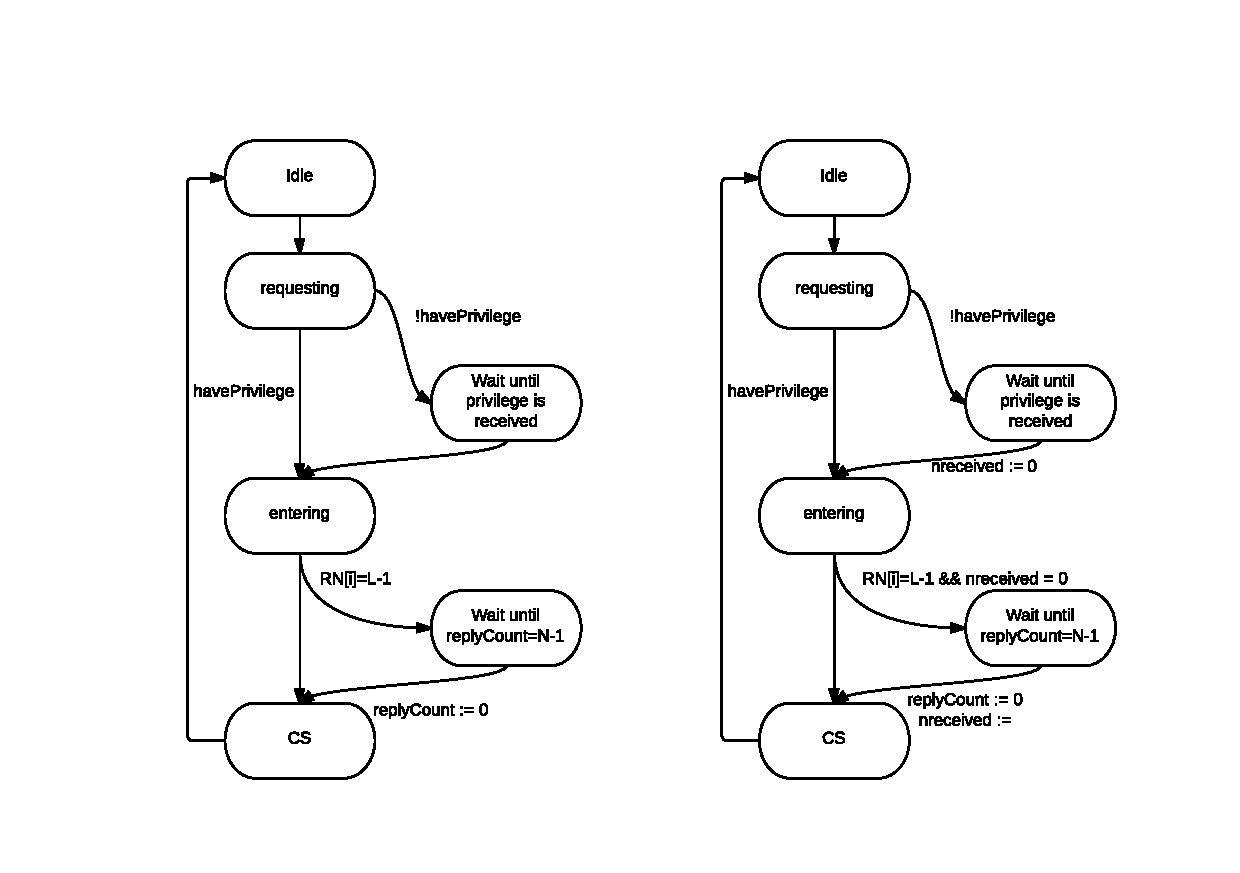
\includegraphics[width=\textwidth]{diagramboth.pdf}
 \caption[Close up of \textit{Hemidactylus} sp.]
   {Simplified flow chart of the SKAM algorithm (left). Flow chart after extending the model with a variable \texttt{nreceived}}
\end{center}
\end{figure}

Using this small extension the model was shown to be free from deadlocks. All further model checking results are based on the deadlock-free model. Note that it has been assumed that a nodes execute infinitely often (at least the node holding the privilege); without this non-termination assumption, a deadlock might occur  \cite{OgataSAL}\cite{OgataMaude}.

\subsection{Remaining Properties}
The results show that mutual exclusion, starvation freedom and freedom of unnecessary delay all hold for the SKAM algorithm. 


\section{Discussion}
????

\section{references}
\begin{thebibliography}{4}

\bibitem{OgataSAL}Ogata, K., Futatsugi, K.: Analysis of the Suzuki-Kasami Algorithm with SAL Model Checkers. In: 
Proceedings of the 2005 The Fifth International Conference on Computer and Information Technology (CIT 05)

\bibitem{OgataMaude} Ogata, K., Futatsugi, K.: Analysis of the Suzuki-Kasami Algorithm with the Maude Model Checker. In: 
Proceedings of the 12th Asia-Pacific Software Engineering Conference (APSEC 05)

\bibitem{Suzuki} Suzuki, I., Kasami, T.: A Distributed Mutual Exclusion Algorithm. In: 
ACM Transactions on Computer Systems, Vol. 3, No. 4, November 1985, Pages 344-349.


\end{thebibliography}

\newpage
\label{ref:SKA}

\begin{lstlisting}[label=some-code,caption=Suzuki and Kazami's algorithm]
const I: Integer;		(* the identifier of this node *)
	var HavePrivilege, Requesting:		bool;
	j, n:	 	integer;
	Q: 		queue of integer;
	RN, LN:	array[l . . N] of integer;

	(* The initial values of the variables are:
	HavePrivilege = true in node 1, false in all other nodes;
	Requesting = false; Q = empty;
	RN[j] = -1, j = 1,2, . . . , N;  	LN[j] = -1, j = 1,2,. . . , N; *)

	procedure Pl;
	begin
		Requesting := true;
		if not HavePrivilege then
		begin
			RN[I] := RN[Z] + 1;
			for all j in 11, 2, . . . , NJ - {Z) do
				Send REQUEST(1, RN[I]) to node j;
			Wait until PRIVILEGE(Q, LN) is received;
			HavePrivilege := true
		end,
	
		Critical Section;

		LN[Z] := RN[Z];
		for all j in 11, 2, . . . , N) - [I) do
			if not in(Q, j) and (RN[jJ = LN[j] + 1) then
				Q := append(Q, j);
		if Q f empty then
		begin
			HavePrivilege := false;
			Send PRIVILEGE(tail(Q), LN) to node head(Q)
		end;
		Requesting := false
	end,

	procedure P2; (* REQUEST(j,n) is received; P2 is indivisible *)
	begin
		RN[j] := max(RN[j],n);
		if HavePrivilege and not Requesting and (RN[j] = LN[j] + 1) then
		begin
			HavePrivilege := false;
			Send PRIVILEGE(Q, LN) to node j
		end
	end,

\end{lstlisting}


\end{document}

